\chapter{脾 大}

脾脏是体内最大的免疫器官和血液滤过、破坏场所,具有免疫、调节血容量、贮血及造血(髓样化生时)等功能。脾脏位于左上腹深部,于腋中线第9~11肋间,前界不超过腋前线,正常情况下肋缘下不能触及。凡在仰卧位或侧卧位在肋缘下触及脾脏均可称为脾大(splenomegaly)。游走脾、左侧胸腔积气或积液、内脏下垂等致脾位置下移均不属脾大。如影像学B超检查显示脾厚度超过4cm或最大长径超过11cm以及左肋缘下探及脾,也可判定为脾大。临床按脾大程度分为:①轻度脾大:深吸气时脾下缘可触及但不超过肋下2cm。②中度脾大:脾下缘超出肋下2cm,在脐水平线以上。③高度脾大,即巨脾:脾下缘超出脐水平线或脾大超出前正中线。

脾大的发病机制:①感染:脾脏具有血液过滤、隔离和清除异物或病原体、产生抗体的功能。当某种病原体如细菌、寄生虫、真菌等侵入人体引起急性感染时,病原体刺激脾脏,脾淋巴细胞、巨噬细胞及血管系统反应性增生,血流量增多而导致脾脏肿大。病原体侵入人体引起慢性感染时,病原体长期反复刺激脾脏或直接引起局部炎症,脾单核巨噬细胞和淋巴细胞明显增生伴纤维组织大量形成,脾脏可呈中度肿大。②脾脏淤血:肝硬化、门静脉、脾静脉栓塞或受压时,脾静脉压力增高,脾脏淤血,静脉窦明显扩张,脾索增宽,红髓网状纤维增生、脾小梁增宽,导致脾大。③脾脏髓样化生:婴儿期正常脾脏已不再具有造血功能,但在骨髓纤维化等时,脾脏可发生髓样化生而恢复造血功能,脾脏红髓造血干细胞、巨噬细胞等增生,造成脾大。④脾脏异常物质沉积:血细胞主要通过脾索、血窦间的基膜小孔进入血窦,再进入脾静脉,这些基膜小孔直径为2~3μm,而红细胞直径为7~9μm,必须通过变形才能通过。但球形红细胞变形能力差,常无法通过,故长期阻滞在脾索而被巨噬细胞破坏,当红细胞内铁粒、变性珠蛋白小体等物质被巨噬细胞剔除后,红细胞才能通过,多次剔除使细胞易发生溶血,含铁血黄素等物质沉积,在脾索中大量被隔离、堆积,脾索和血窦扩张、充血,内皮细胞增生,导致脾大。⑤肿瘤细胞浸润:白血病、恶性淋巴瘤、恶性组织细胞病及真性红细胞增多症时肿瘤细胞可在脾脏内浸润增生,造成脾大。引起脾大的疾病很多,按病因可分为感染性脾大与非感染性脾大两大类(表\ref{tab31-1})。

脾大患者在临床诊断思路方面要着重注意以下几点:

\section{【病史】}

详细询问病史对脾大疾病的诊断常能提供重要线索,除一般询问外,应特别询问下列情况:

\subsection{(一)注意传染病和流行病}

注意患者所在地区、患者籍贯、旅居地,发病季节,询问有关接触史、预防接种史和当地流行情况。患者如居住于疟疾高发区应考虑疟疾的可能,在长江沿岸的血吸虫病区,无其他原因可解释的脾大且有疫水接触史者应疑及血吸虫病。

\subsection{(二)起病缓急}

急性起病、脾进行性肿大应多考虑急性感染、恶性血液病。慢性感染性疾病起病缓慢。自幼脾大伴贫血、黄疸、浓茶尿应疑及遗传性溶血性贫血。

\subsection{(三)传染病史、家族史}

既往患过肝炎,症状未愈且出现明显脾大应注意有无肝硬化,有否疟疾、血吸虫病等病史。有无海洋性贫血、血红蛋白病等家族史。

\subsection{(四)重视伴随症状}

脾大伴不规则发热、进行性无痛性浅表淋巴结肿大应考虑恶性淋巴瘤。脾大伴发热、皮疹、关节痛应注意有无自身免疫病。脾大伴发热、贫血、出血倾向者应注意有无恶性血液病、重症感染。脾大伴高热寒战者,多属感染性疾病或恶性血液病合并感染。脾大伴皮肤黄染、发热应注意重症肝炎、急性溶血、钩端螺旋体病。

\section{【体征】}

\subsection{(一)一般检查}

注意有无发热;注意皮肤有无苍白、紫癜、瘀斑,黏膜有无苍白、出血。脾大伴急性发热、贫血、出血点等应考虑有无败血症、亚急性感染性心内膜炎、恶性血液病、SLE。急性感染一般呈急性面容。伤寒、副伤寒患者表情淡漠,呈“伤寒面容”。面部蝶形红斑提示活动性SLE。真性红细胞增多症患者结膜充血,面色绛红,口唇和耳垂发绀。斑疹伤寒和恙虫病者可呈醉酒面容。皮肤或软组织脓肿可为败血症的来源。胸骨下段压痛强烈提示白血病。发现心脏明显器质性杂音需注意感染性心内膜炎。

\begin{longtable}{c}
 \caption{脾大疾病的分类}
 \label{tab31-1}
 \endfirsthead
 \caption[]{脾大疾病的分类}
 \endhead
 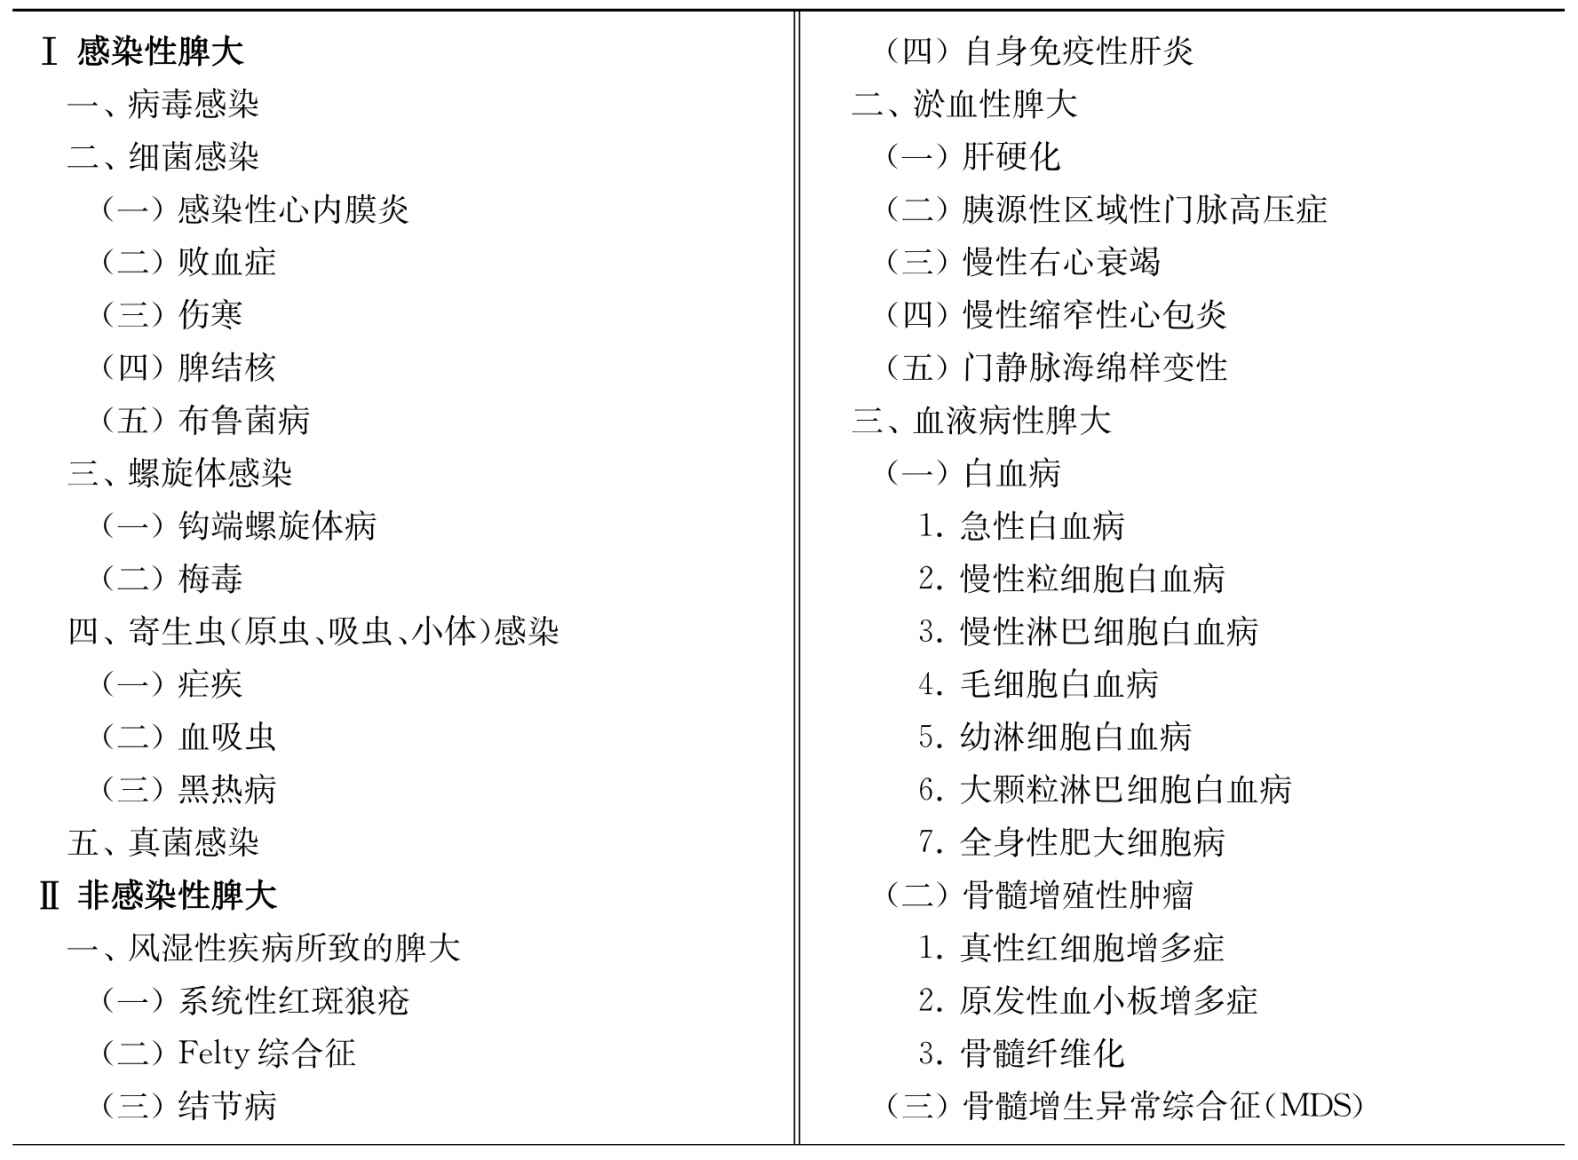
\includegraphics[width=\textwidth,height=\textheight,keepaspectratio]{./images/Image00159.jpg}\\
 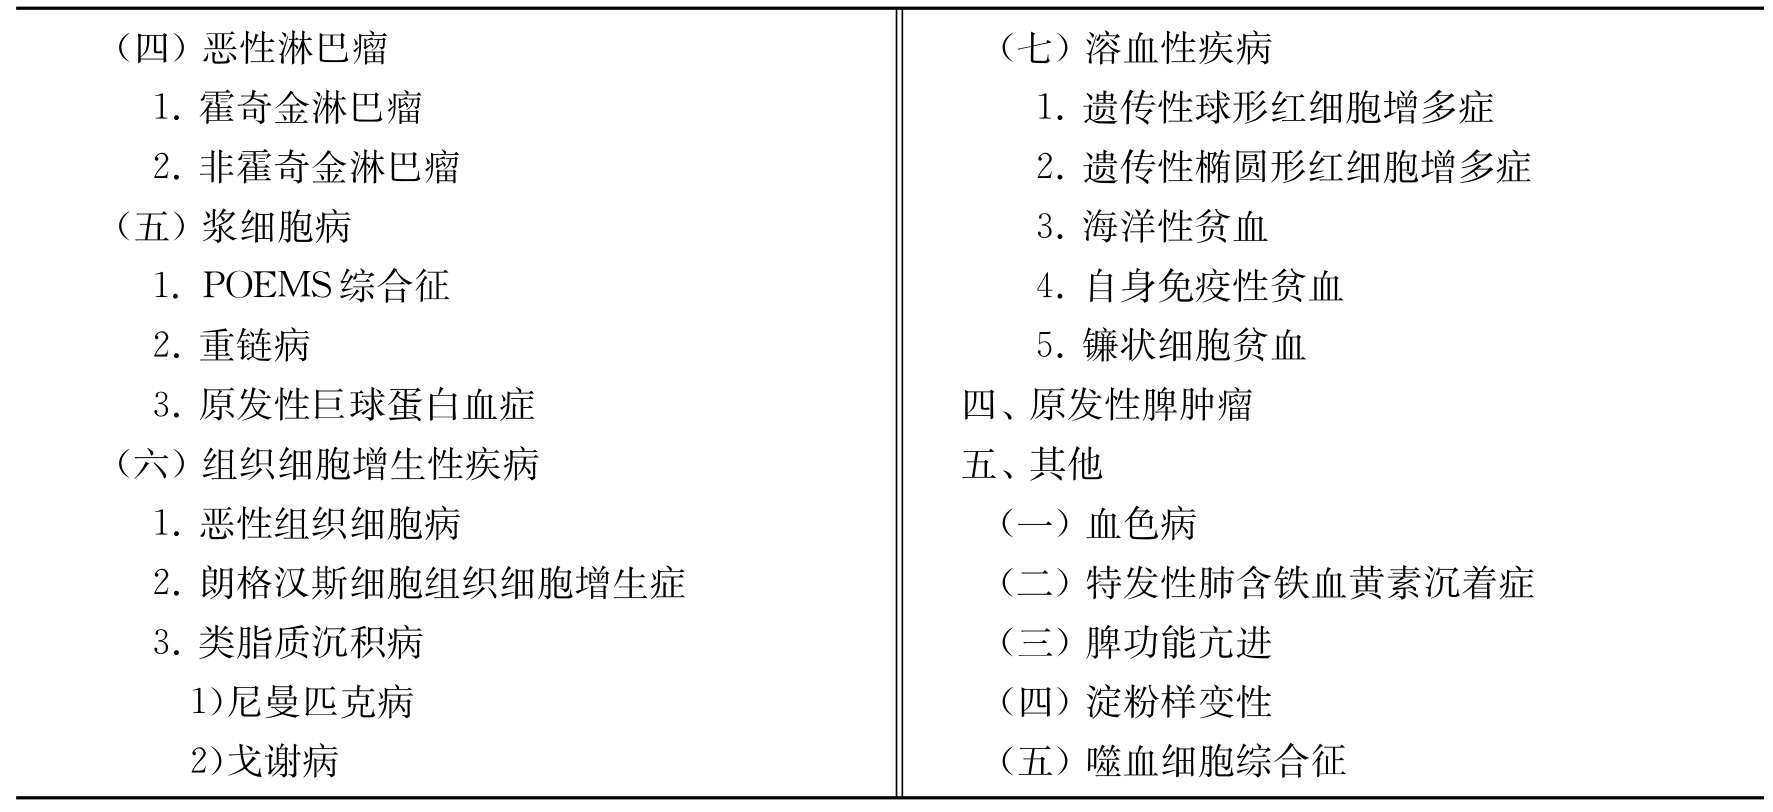
\includegraphics[width=\textwidth,height=\textheight,keepaspectratio]{./images/Image00160.jpg}
 \end{longtable}

\subsection{(二)淋巴结}

注意全身浅表淋巴结有无肿大。脾大伴全身淋巴结肿大应注意有无传染性单核细胞增多症、急、慢性淋巴细胞性白血病、恶性淋巴瘤、急性髓系白血病、朗格汉斯组织细胞增生症、组织细胞坏死性淋巴结炎、急性粟粒型结核等。肿大的淋巴结质软、有压痛、可移动支持急性感染性疾病;质韧实、无压痛且富有弹性提示恶性淋巴瘤;质坚硬无压痛,移动性差提示淋巴结转移癌。

\subsection{(三)肝脏}

肝脾均大,需注意有无慢性肝病、肝硬化、右心衰竭、各种传染病、血液病、类脂质沉积症等。

\subsection{(四)脾脏}

注意脾大程度、质地、有无摩擦感、有无压痛。轻度脾大、质软、有轻度压痛提示急性感染性疾病;轻度脾大、质中、无明显压痛见于SLE、MDS、真性红细胞增多症、原发性血小板增多症、多发性骨髓瘤、恶性组织细胞病、慢性溶血性疾病、血色病、结节病、急性髓系白血病等。中度脾大、质地较硬、无明显压痛见于脾结核(部分可有压痛)、部分慢性疟疾、少数慢性粒细胞白血病和大多数慢性淋巴细胞白血病、部分慢性血吸虫病、门脉性肝硬化、脾门静脉血栓形成、部分毛细胞白血病、部分幼淋细胞白血病、急性淋巴细胞白血病、恶性淋巴瘤、朗格汉斯细胞组织细胞增生症、部分真性红细胞增多症、原发性血小板增多症、部分遗传性溶血性贫血病等。高度脾大(巨脾)、质较硬、无压痛提示部分慢性疟疾、部分血吸虫病、大多数慢性粒细胞白血病、毛细胞白血病、部分幼淋细胞白血病、骨髓纤维化、少数恶性淋巴瘤(如脾淋巴瘤)、黑热病、镰状细胞性贫血、脂质沉积病等。脾质地软、有囊性感见于脾囊肿。脾压痛明显有摩擦音见于脾周围炎、脾梗死。脾大有压痛见于脾脓肿、脾梗死。脾表面不光滑者应注意脾恶性肿瘤。

\section{【实验室和特殊检查】}

\subsection{(一)血象}

\subsubsection{1.白细胞总数及分类计数}

多数病毒感染白细胞总数正常。白细胞增多、分类以中性粒细胞为主常见于急性化脓性细菌感染、钩端螺旋体病、急性血吸虫病。白细胞增多且原始及幼稚细胞超过20\%者强烈提示急性白血病。白细胞减少见于伤寒、副伤寒、病毒感染、立克次体感染、疟疾、急性非白血病性白血病、恶性组织细胞病、风湿性疾病、脾功能亢进、骨髓增生异常综合征、严重感染而反应性差者。嗜酸性粒细胞增多见于寄生虫感染如急性血吸虫病、肝吸虫病、恶性淋巴瘤、骨髓增殖性肿瘤(包括慢性粒细胞白血病)等。嗜碱性粒细胞增多见于慢性粒细胞白血病和嗜碱性粒细胞白血病。单核细胞增多见于传染性单核细胞增多症、组织细胞坏死性淋巴结炎、某些活动性结核病、亚急性细菌性心内膜炎,急性单核细胞白血病、慢性粒-单核细胞白血病等。严重感染时中性粒细胞胞质内可见中毒颗粒、嗜碱性包涵体(Dohle小体)、核变性及空泡变性等。异常淋巴细胞>10\%应注意传染性单核细胞增多症。血涂片见疟原虫可确诊疟疾。

\subsubsection{2.红细胞计数与血红蛋白量}

急性严重感染,如败血症、感染性心内膜炎、粟粒型结核,患者可在短期内出现贫血,而慢性感染、脾功能亢进、溶血性贫血、风湿性疾病等,可出现轻至中度贫血,而恶性血液病常出现中至重度贫血。红细胞>7.0×10\textsuperscript{12}
/L或血红蛋白>200g/L提示真性红细胞增多症。

\subsubsection{3.血小板计数}

血小板重度增多,超过1000×10\textsuperscript{9}
/L提示原发性血小板增多症。血小板减少见于严重感染、脾功能亢进、恶性血液病、骨髓增生异常综合征、系统性红斑狼疮等。

\subsubsection{4.全血细胞减少}

全血细胞减少可见于严重感染、败血症、脾功能亢进、系统性红斑狼疮、骨髓增生异常综合征、急性非白血病性白血病、恶性组织细胞病、急慢性肝病等。

\subsection{(二)骨髓象}

多次、多部位骨髓穿刺均干抽,骨穿进、出针费力,应疑及骨髓纤维化,需作骨髓活检证实。骨髓有核细胞极度或明显增生,早幼粒以下各阶段粒细胞均增生,伴嗜酸粒及嗜碱性粒细胞增多、中性粒细胞碱性磷酸酶活性明显减低或缺如,提示为慢性粒细胞白血病。原始粒(单核或淋巴)细胞+早幼粒(或幼稚单核或淋巴细胞)>20\%应诊断为急性白血病。骨髓见组织细胞增多且呈异质性,特别是同时可见到多核巨细胞时应考虑恶性组织细胞病。骨髓呈全骨髓增生伴巨核细胞增多应注意原发性血小板增多症、真性红细胞增多症。如见到疟原虫则疟疾的诊断可成立;如见到利什曼原虫则可确诊黑热病。骨髓二系或以上病态造血是骨髓增生异常综合征的佐证。骨髓见戈谢细胞应注意戈谢病。见尼曼匹克细胞应考虑尼曼匹克病。

\subsection{(三)大便}

集卵法检查到华支睾吸虫卵可诊断肝吸虫病、检查到血吸虫卵可确诊血吸虫病。

\subsection{(四)病原体与血清学检查}

疑为急性感染性脾大时应适时取血、骨髓液、痰、尿培养等以利寻找病原对因治疗。同时可行血清学检查如肥达反应、外-斐反应、嗜异性凝集试验、EB病毒抗体、钩端螺旋体检测、血吸虫病有关抗体、抗原检测。血清蛋白免疫固定电泳和尿本周蛋白电泳可确定有无多发性骨髓瘤、巨球蛋白血症。抗核抗体、抗双链DNA抗体、抗Sm抗体、补体C3、补体C4、免疫球蛋白定量测定有助于风湿性疾病系统性红斑狼疮的诊断。肝炎系列血清学检查可诊断各型肝炎病毒感染的有无。

\subsection{(五)影像学检查}

腹部B超可测定肝脾大小,有无脾囊肿、脾脓肿、脾占位性病变。有无腹膜后淋巴结肿大。彩色多普勒可查明门脉和脾静脉宽度、血管内有无栓塞等。X线胸片可明确肺部有无感染、肿块,纵隔淋巴结有无肿大,肋间、胸骨、胸椎有无破坏。食管吞钡见胃底、食管静脉曲张支持门脉高压的诊断。必要时可行CT或MRI检查。PET-CT显像能同时提供功能和解剖信息,大大提高了诊断的准确性。

\subsection{(六)病理学检查}

脾大伴淋巴结肿大者可行淋巴结活检以明确诊断,可确诊恶性淋巴瘤、恶性组织细胞病、朗格汉斯细胞组织细胞增生症、组织细胞坏死性淋巴结炎等。脾大患者凝血功能无异常者可在B超引导下行脾穿刺活检,可确诊脾结核、恶性淋巴瘤、脾囊肿、脾原发肿瘤、淀粉样变性、黑热病、恶性组织细胞病等。不明原因发热伴脾脏肿大脾切除病理诊断率约为64\%~77\%左右,对于诊断性脾切除术的手术指征并没有明确的标准。

\subsection{(七)其他}

如PPD皮试协诊粟粒型肺结核。溶血试验诊断各种溶血性疾病。Ph染色体检测阳性、BCR/ABL融合基因检测阳性可确诊慢性粒细胞白血病。肝功能检查肝功能损害,白蛋白(A)减低,球蛋白(G)升高、A/G比值倒置、凝血功能检查示凝血酶原时间延长提示重症肝病、肝硬化。

\protect\hypertarget{text00245.html}{}{}

\section{108 感染性脾大}

\subsection{一、病毒感染}

传染性单核细胞增多症的主要症状为发热、咽痛、皮疹、淋巴结肿大(质软有轻压痛)、脾大(多为轻度质软有轻压痛)。白细胞总数可升高也可正常或减低,淋巴及单核细胞增多,异常淋巴细胞>10\%,肝功能异常。血清抗体(此抗体抗羊红细胞、不被豚鼠肾细胞吸收)嗜异性凝集试验在起病4~5天至两周内可阳性,EB病毒抗体尤其是VCA-IgM阳性。多数病程为两周,有内脏损害的重症患者病程延长至数月。

\subsection{二、细菌感染}

\subsubsection{(一)亚急性感染性心内膜炎}

有先天性或风湿性瓣膜性心脏病史。可有发热、乏力、肌肉关节疼痛。约60\%以上患者有轻度脾大、质软有轻压痛,伴脾梗死者左上腹有剧痛。可有皮肤瘀点及其他脏器梗死的表现。超声心动图检查可发现瓣膜赘生物、反复血培养(包括细菌、真菌等)可获阳性结果。

\subsubsection{(二)败血症}

起病多急骤、寒战后高热、大汗,皮肤可出现瘀点。脾大一般为轻度,且可有轻压痛。如未接受有效的治疗,体内多处可出现转移性脓肿,疑为此症应多次血培养(包括细菌、厌氧菌、真菌),用抗生素前、寒战时抽血作培养可望提高阳性率,必要时可作骨髓液培养找病原体,阳性时作药敏试验。

\subsubsection{(三)伤寒}

典型病例初期体温逐步上升,5~7天后呈高热稽留不退约二周,中毒症状较严重,相对缓脉,有显著神经系统症状,表情淡漠、嗜睡甚至谵妄、昏迷,腹胀、轻度腹痛。脾大多为轻度,质软、可有轻度压痛。部分病例有蔷薇疹。肥达试验在本病起病一周后即可出现阳性反应,“O”抗体1∶80以上阳性,H在1∶160以上,若动态观察,抗体滴度逐步上升诊断意义更大。

\subsubsection{(四)脾结核}

主要为全身粟粒性结核所致。起病缓慢,多有发热、苍白、乏力、消瘦、厌食、衰弱、体重减轻、恶心、腹胀、腹痛。脾大多为中度,质较韧实,压痛不明显,常伴肝大。部分病例可找到脾外结核,PPD皮试多数阳性,少数阴性。在有条件的医院,诊断有困难时可在B超指引下行脾穿刺活检术,有助确诊。可疑病例试验性抗结核治疗如疗效明显,包括全身症状减轻、热退、脾(及肝)明显缩小亦可确定诊断。

\subsubsection{(五)布鲁菌病}

由布鲁菌属引起,多有从事屠宰、饲养、皮毛加工与家畜及畜产品接触史,3~6月份多见,临床常见表现有发热、食欲不振、多汗、倦怠无力等,伴咳嗽、咳痰、头痛、心悸、关节疼痛或肿胀、肝脾大、肝肾功能异常、血沉、C反应蛋白升高等。布鲁菌凝集试验阳性,静脉血或穿刺液培养阳性,经细菌学鉴定为布鲁菌可诊断。

\subsection{三、螺旋体感染}

\subsubsection{(一)钩端螺旋体病}

脾大在本病无重要鉴别诊断意义。本病早期骤发高热、头痛、全身肌痛尤其是腓肠肌剧痛、明显压痛,中期的多器官(肺、肝、肾、脑)损害,晚期的后发热、眼后发症、神经系统后发症,白细胞增多,贫血和血小板减少,全身浅表淋巴结肿痛但局部皮肤无充血、发炎,也不化脓等临床特点。病原体分离、动物接种和酶联免疫吸附试验或钩端螺旋体IgM抗体检查可明确诊断。

\subsubsection{(二)梅毒}

脾大对梅毒无重要鉴别诊断意义。梅毒的诊断主要依据:①不洁性交史。②各期临床表现,如初期腹股沟淋巴结无痛性肿大、硬性下疳,二期全身性轻至中度淋巴结肿大,肿大的淋巴结无压痛、不粘连,各期梅毒疹,不加热的血清素(USR)试验阳性,扁平湿疣、下疳或黏膜损伤活组织暗视野直接镜检可发现梅毒螺旋体。

\subsection{四、寄生虫(原虫、吸虫、小体)病}

\subsubsection{(一)疟疾}

间日疟、三日疟的典型发作为寒战、高热、盛汗三阶段,每隔48、72小时重复发作,常伴寒战、畏寒、头痛、肌痛、恶心、呕吐、烦渴等。脾渐增大,病程越长,发作次数越多,脾大越显著,晚期形成巨脾。诊断根据流行区居住史、典型临床症状、脾大、血涂片查见疟原虫等。

\subsubsection{(二)血吸虫病}

脾明显大多见于慢性血吸虫病。慢性血吸虫病病程由数月至数十年不等。巨脾多因多次反复小量感染血吸虫引起。临床表现为肝硬化、腹胀、腹泻、食欲缺乏、营养不良、肝脾大(肝大不如脾大明显)、常有腹水、上消化道出血。诊断依据:①流行区疫水接触史;②临床表现;③兼用沉淀集卵法及毛蚴孵化法粪便查虫卵,反复进行可提高检出率;④血吸虫抗原皮内试验阳性;⑤直肠黏膜活检发现血吸虫卵。

\subsubsection{(三)黑热病}

旧称内脏利什曼病。起病缓慢,早期发热、畏寒、出汗,热型不定,典型为双峰热,发热可反复发作数月至一年以上。脾脏随病程迁延而逐渐增大,终至巨脾,常伴全血细胞减少,血浆球蛋白增高。诊断依据:①流行区居住史。②长期发热、脾大、全血细胞减少,多克隆高丙种球蛋白血症等临床特点。③骨髓涂片或肝、脾、淋巴结穿刺涂片找到利什曼小体可确诊。补体结合试验阳性率90\%以上,阳性有助于诊断。

\subsection{五、真菌感染}

深部真菌感染可引起全身各个脏器的广泛播散,肝脾是最常受累器官之一。组织胞浆菌病临床表现主要为发热、寒战、咳嗽、咳痰、胸痛、腹痛等,可合并神经系统症状或出现淋巴结肿大、贫血、体表包块,可以发生巨脾,患者多有基础免疫受抑情况,诊断主要依据骨髓检查发现组织胞浆菌。播散性肝脾念珠菌病表现为持续性发热、广谱抗生素治疗无效、上腹胀痛、恶心、呕吐、肝脾大伴叩痛,B超或CT主要表现为肝脾多发性圆形或椭圆形低密度影,部分可见典型牛眼征。肝脾穿刺组织培养和病理学有念珠菌感染证据支持诊断。

\protect\hypertarget{text00246.html}{}{}

\section{109 非感染性脾大}

\subsection{109.1 风湿性疾病}

\subsubsection{一、系统性红斑狼疮}

本病多见于青年女性,常累及多个器官,包括皮肤、肌肉、关节、浆膜、心脏、肾脏、消化道、中枢神经系统、眼等。脾大仅见于20\%左右患者,多为轻度肿大且多无压痛。对本病的鉴别诊断意义不大。肝大及肝功能损害见于约30\%患者。诊断依据临床表现,面部蝶形红斑,抗核抗体高滴度阳性,抗Sm抗体阳性(特异性98\%,敏感性30\%),抗双链DNA抗体阳性(特异性95\%,敏感性70\%),皮肤狼疮带阳性,低补体C4等。

\subsubsection{二、Felty综合征}

临床表现为进行性类风湿关节炎。脾常中度大,质较韧实而无压痛。浅表淋巴结及肝轻度大,有脾功能亢进的症状、体征及骨髓象表现。

\subsubsection{三、结节病}

本病主要临床表现为咳嗽、胸闷、气促、发热、浅表淋巴结肿大,半数左右患者可有肝脾轻度大,质中而无压痛。但脾大在本病无重要鉴别诊断意义。本病诊断主要依据:①X胸片示双侧肺门及纵隔对称性淋巴结肿大,伴或不伴有肺内网状、结节状、片状阴影,PET-CT成像SUV值往往升高,与转移癌、淋巴瘤十分相似,难以鉴别。②组织活检特征为非干酪样坏死性类上皮细胞肉芽肿,证实或符合结节病,并需排除其他肉芽肿性疾病。此外,血清血管紧张素转换酶活性升高、PPD皮试阴性或弱阳性以及高血钙、高尿钙、碱性磷酸酶增高、血浆免疫球蛋白增高等也有助于本病的诊断。

\subsubsection{四、自身免疫性肝炎}

本病女性易患,主要表现为乏力、食欲减退、上腹部不适、发热,常有蜘蛛痣、高球蛋白血症、伴其他自身免疫性疾病等,大多数患者存在一种或多种高滴度的自身抗体,如抗核抗体、肝肾微粒体抗体、平滑肌抗体等。肝外表现可有关节炎、女性闭经、男性乳房发育、桥本甲状腺炎等,腹部CT表现为肝脏质地不均、密度减低、肝硬化,胆囊壁增厚、胆囊结石、脾脏增大,腹腔多发淋巴结,腹腔积液等。特征性病理组织学表现是界板炎症,可出现肝脏纤维化和肝硬化的病理表现。

\protect\hypertarget{text00247.html}{}{}

\subsection{109.2 淤血性脾大}

\subsubsection{一、肝硬化}

门脉性肝硬化多数伴有脾大,脾大常与肝大成反比,即肝愈缩小时脾大往往愈显著。坏死后性肝硬化也常伴脾大,一般为轻度。胆汁性肝硬化的脾大大多为轻度或中度。诊断主要依据:①病史;②乏力、食欲缺乏、恶心、右上腹不适、消瘦等肝功损害的症状;③门脉高压表现:脾大、胃底或(及)食管静脉曲张、腹水(胸腔积液、水肿);④肝功能损害实验室检查结果,特别是低白蛋白血症和高球蛋白血症(A/G比值倒置);⑤肝穿刺活检为金标准,需一定的条件和技术水平。原发性胆汁性肝硬化常伴有其他自身免疫性疾病,如干燥综合征、自身免疫性甲状腺炎等,免疫学指标血清抗线粒体抗体(AMA)或AMA-M2亚型阳性。

\subsubsection{二、胰源性区域性门脉高压症}

本病最常见的原因是慢性胰腺炎和胰腺假性囊肿,其次为胰腺肿瘤。主要表现为胰腺疾病和门脉高压两组症候群,首发症状以腹痛、腹泻、黑便、贫血多见,部分患者无任何症状或仅有腹痛、消瘦和上腹部肿块等胰腺疾病的症状,腹水较少发生,脾亢多为轻到中度,肝功能多正常。本病诊断的金标准是腹部血管造影和经皮穿刺门静脉造影,腹腔动脉造影见静脉像的脾静脉不显影,脾静脉与门静脉间其他侧支显影,肠系膜上动脉造影的静脉像见正常的门静脉显影,冠状静脉不显影,选择性脾动脉造影示脾静脉阻塞。

\subsubsection{三、慢性右心衰竭}

心瓣膜病并发慢性右心衰竭时,脾脏通常不仅不因静脉淤血而肿大,反而常因缺氧而致脾脏萎缩,但发展至心源性肝硬化时则多有脾大。

\subsubsection{四、慢性缩窄性心包炎}

慢性缩窄性心包炎约50\%病例具有脾大。

\subsubsection{五、门静脉海绵样变性}

门静脉海绵样变性是由于门静脉主干或其分支部分或完全血流受阻,机体为减轻门静脉高压,在肝门区形成大量侧支血管丛,是形成肝前型门静脉高压症的原因之一。临床少见,分为原发性和继发性,前者主要是肝门及其分支门静脉管腔的缺失,结构先天发育异常,狭窄或闭锁所致;后者多继发于急性门静脉血栓或癌栓后,其次与门静脉纤维组织炎、各种凝血系统疾病、消化系统疾病及外界压迫有关。大多数患者胃镜检查可见食管胃底静脉曲张,肝脏本身常无明显异常改变,肝功能多不受影响,患者不易出现黄疸和腹水,门静脉海绵样变性一般通过影像学检查即可明确。

\protect\hypertarget{text00248.html}{}{}

\subsection{109.3 血液病}

\subsubsection{一、白血病}

\paragraph{(一)急性白血病}

起病急,进展快,早期即可有高热、贫血、出血。肝、脾、淋巴结可肿大,以急性淋巴细胞白血病较显著。胸骨下段有压痛具诊断意义。外周血白细胞可明显增高或正常亦可减少,增高者分类可见大量原始及幼稚细胞。骨髓检查最具诊断意义:骨髓中原始+早幼粒(幼稚单核或淋巴)细胞≥20\%,具异质性(形态学上畸形明显)即可成立诊断。组织化学染色、免疫学分型、细胞遗传学检查及分子生物学检测可进一步分型确诊。

\paragraph{(二)慢性粒细胞白血病}

慢性期无症状或低热、乏力、多汗、上腹胀、体重减轻、胸骨中下段压痛。脾大多较显著,多为巨脾,除非合并脾周围炎,一般质较硬而无压痛。血象白细胞明显升高,多为(100~300)×10\textsuperscript{9}
/L,分类粒细胞占绝大多数,可见早幼粒以下各阶段粒细胞增多,伴嗜酸性、嗜碱性粒细胞同时明显增多,多数有轻度贫血和血小板增多。骨髓增生明显活跃或极度活跃,以粒系占绝大多数,分类似外周血象。红细胞系比例明显减低、巨核细胞及血小板常增多。粒细胞碱性磷酸酶活性明显降低或缺如。患者Ph染色体或BCR/ABL融合基因阳性。

\paragraph{(三)慢性淋巴细胞白血病}

多于中老年发病,早期多无症状,病情进展慢,进展中淋巴结、肝脾渐大。脾大多为中度,个别晚期可极度大,质中至较硬,无压痛。贫血和出血见于晚期。血象白细胞增多,多为(30~80)×10\textsuperscript{9}
/L,分类计数见60\%以上为成熟小淋巴细胞及少量幼稚淋巴细胞。骨髓示小淋巴细胞明显增多,>40\%,可见少量幼稚淋巴细胞。

\paragraph{(四)毛细胞白血病}

少见。发病年龄多在40岁以上,常有贫血症状,出血常不严重,易并发感染。体征脾大突出,多为巨脾,质较硬而无压痛。血象示贫血、血小板减少,白细胞多为减少(全血细胞减少),但也可正常或增高,分类以淋巴细胞为主,可见数量不等的毛细胞(白细胞>10×10\textsuperscript{9}
/L时,毛细胞常占30\%以上)。骨髓增生明显活跃,以淋巴细胞为主,毛细胞≥30\%。毛细胞中等大小,胞浆量多,呈灰蓝色,胞浆周边不规则,有许多纤毛状突起,形似伪足,胞浆与胞核之间有明显淡染区,核染色质疏松,多数未见核仁,少数可见1~2个核仁,透射电镜可见这些细胞质有核糖体板复合物。细胞化学染色、酸性磷酸酶染色阳性且不被酒石酸盐所抑制。毛细胞除具B细胞免疫表型(CD19\textsuperscript{+}
、CD20\textsuperscript{+}
)外,细胞膜单克隆抗体典型表型(CD11c、CD25以及CD103)阳性,TPA反应阳性。

\paragraph{(五)幼淋细胞白血病}

幼淋细胞白血病好发于60岁以上的老人,中位年龄70岁,其主要临床表现为发热、多汗、乏力、消瘦、腹胀、脾明显肿大,周围淋巴结不增大或轻度增大。诊断标准为血液循环的淋巴细胞中幼淋细胞比例>55\%。多数患者WBC>100×10\textsuperscript{9}
/L,部分患者伴有贫血和血小板减少。幼淋细胞外形较大,大约是小淋巴细胞的两倍大小,核质比例高,有少量的淡蓝色胞浆和圆形的核,核染色质呈中度块状,有一个明显的中央核仁。这种细胞与一般所见的急性淋巴细胞白血病的幼稚淋巴细胞不同(有一至多个核仁,核染色质均匀细致),应特别注意区分。根据免疫分型分为B细胞和T细胞-幼淋细胞白血病两大类型,临床以前者多见。

\paragraph{(六)大颗粒淋巴细胞白血病}

本病与急性淋巴细胞白血病不同的是,外周血与骨髓分类大颗粒白血病性淋巴细胞(体积大,胞浆丰富且多含有粗大的嗜苯胺蓝颗粒)占多数,常无浅表淋巴结肿大,而脾大突出,可为巨脾,质较硬而无压痛。大颗粒细胞可为CD3\textsuperscript{-}
的NK细胞或T细胞。T细胞型常伴中性粒细胞减少、红细胞增生不良和类风湿关节炎(但不属Felty综合征),常见免疫表型为CD3\textsuperscript{+}
、CD4\textsuperscript{-} 、CD8\textsuperscript{+}
、CD16\textsuperscript{+} 、CD56\textsuperscript{-}
、CD57\textsuperscript{+} 、TCRαβ\textsuperscript{+} 。

\paragraph{(七)全身性肥大细胞病}

该病的首发症状是多发性皮肤色素性荨麻疹,以后波及至淋巴结、肝、脾及胃肠等内脏,表现为淋巴结、肝、脾大。脾大较突出,常为巨脾。累及骨髓则表现为贫血、血小板减少,但外周血白细胞常超过30×10\textsuperscript{9}
/L,肥大细胞常占50\%以上,此时称为组织嗜碱细胞(肥大细胞)白血病。累及胃肠则多表现为腹痛、腹泻。肥大细胞体积较大,无纤毛,胞浆充满嗜苯胺蓝颗粒。此外,肥大细胞产生的组胺等可引起潮红、哮喘、面部四肢水肿、头痛、甚至休克,是本病的特征,具鉴别诊断意义。

\subsubsection{二、骨髓增殖性肿瘤}

\paragraph{(一)真性红细胞增多症}

特点为多血症,如皮肤、黏膜绛红、脾可肿大(多为轻至中度、晚期伴骨髓纤维化时可为巨脾)。红细胞增多(男>6.5×10\textsuperscript{12}
/L,女>6.0×10\textsuperscript{12}
/L)。血红蛋白增多(男>180g/L,女>170g/L)。\textsuperscript{51}
Cr标记红细胞容量增加(男>36ml/kg,女>32ml/kg,血氧饱和度≥92\%)。如无条件测红细胞容量,则血红蛋白增多以男>200g/L,女>190g/L为宜。白细胞或(及)血小板轻度增高。骨髓示全骨髓三系细胞均增生,尤以红系明显。中性粒细胞碱性磷酸酶积分>100分,血清维生素B\textsubscript{12}
>900pg/ml(>666pmol/L)。

\paragraph{(二)原发性血小板增多症}

主要有出血、血栓形成引起的症状和体征,脾大(可轻~高度)。血小板计数常>1000×10\textsuperscript{9}
/L。白细胞总数可轻度增多。血涂片可见大片成堆血小板,巨大血小板易见。骨髓巨核细胞增多,体大浆多,血小板大片成堆分布。

\paragraph{(三)骨髓纤维化}

中位发病年龄为65岁,主要的临床特点是:①巨脾是本病的特征,约50\%的病例于确诊时脾大已达盆腔,右缘超过腹中线,肿大的脾质多坚硬,表面光滑,无触痛。50\%~66\%的患者有轻到中度的肝大。②贫血、外周血涂片可见幼稚粒细胞及有核红细胞,可见泪滴形红细胞,血小板计数可正常或减少。③骨髓穿刺觉骨质坚硬,多次“干抽”或呈“增生低下”。④肝、脾、淋巴结病理检查示有髓外造血灶。⑤骨髓活检示胶原纤维或(及)网状纤维明显增生。其他常见的不典型症状有乏力、多汗、消瘦、上腹部闷胀感,严重者有骨痛、发热、贫血、出血、痛风性关节炎等。少数患者并发肾结石、听力减退、肺功能减退、腹水、血尿、尿频等。晚期还可有皮肤紫癜、瘀斑,面色苍白及下肢水肿表现。

\subsubsection{三、骨髓增生异常综合征(MDS)}

临床以贫血为主要表现,兼有出血或(及)发热。体征可有轻度脾大。血象呈全血细胞减少或一至二系细胞减少,有巨大血小板、巨大红细胞、有核红细胞、粒细胞核不分叶或分叶过多等病态造血表现。骨髓示增生活跃(少数增生减低)以红系增生较明显,三系或任何二系病态造血(注意除外红白血病、骨髓纤维化、慢性粒细胞白血病等引起的病态造血)。

\subsubsection{四、恶性淋巴瘤}

分霍奇金淋巴瘤和非霍奇金淋巴瘤两大类。

\paragraph{(一)霍奇金淋巴瘤}

无痛性淋巴结肿大,不同部位的淋巴结肿大可能引起的相应部位的器官压迫症状,可伴发热、盗汗、消瘦、皮肤瘙痒等全身症状。血象可有嗜酸性粒细胞增多、可出现贫血。晚期侵犯肝、脾、骨、骨髓等结外组织并引起相应症状、血象可出现全血细胞减少或1~2系细胞减少。确诊需靠病理诊断,或骨髓象发现典型Reed-Sternberg细胞。少数患者可并发Coombs试验阳性或阴性的溶血性贫血。

\paragraph{(二)非霍奇金淋巴瘤}

临床表现以无痛性淋巴结肿大为主,韦氏咽环、胃肠道、睾丸、腹腔内淋巴结病变均较霍奇金淋巴瘤多见。往往一开始即为全身性广泛分布的病变,临床谱广,部分患者表现为长期或周期性发热,常侵犯骨髓而可发展为淋巴瘤细胞性白血病。确诊依靠淋巴结或受犯组织病理检查或骨髓见淋巴瘤细胞。当临床上高度怀疑淋巴瘤时,不能凭一两次病理检查阴性而轻易放弃诊断。

\subsubsection{五、浆细胞病}

\paragraph{(一)POEMS综合征}

本病主要临床特点包括:慢性进行性对称性肢体远端感觉运动障碍,病变为神经轴突变性及节段性脱髓鞘改变;肝脾及淋巴结肿大;内分泌功能障碍,以男性乳房增大和性功能减退、女性闭经、糖尿病、甲状腺功能减退症多见;血清中单克隆免疫球蛋白(M蛋白),多为I
gG及IgA,IgM少见,轻链多为λ型;皮肤病变以弥漫性色素沉着最为常见。尚有全身性水肿包括两下肢水肿、胸腔积液、腹水、心包积液、视乳头水肿、低热、多汗、多毛、杵状指或红细胞、血小板增多等表现。但几个主要临床表现可以不同时出现,其中多发性周围神经及异常M蛋白血症为诊断必备条件。

\paragraph{(二)重链病}

本病罕见,本病分γ、α、μ、δ四种类型。各型的确诊均依赖免疫电泳证实仅有某一单克隆重链而轻链缺如。

\paragraph{(三)原发性巨球蛋白血症}

本病的特点是IgM增高引起血液黏滞度增高、眼底出血或静脉曲张,全血细胞减少而脾大突出,血清IgM>10g/L,骨髓、肝、脾、淋巴结中有淋巴样浆细胞浸润。此外,常有中枢或(及)周围神经系统症状,如脑血管意外,弥漫性或局灶性脑病症状、蛛网膜下腔出血、多发性神经炎以及雷诺现象。

\subsubsection{六、组织细胞增生性疾病}

\paragraph{(一)恶性组织细胞病}

起病急骤,进行性衰竭,长期高热,淋巴结、肝、脾大,病程中常出现黄疸、浆膜腔积液、皮肤损害、出血等症状。血象示全血细胞减少,血涂片偶可见异常组织细胞。确诊依据以上临床表现,加上骨髓涂片及淋巴结、肝、脾活检可见较多异常组织细胞、特别是多核巨组织细胞。近年对恶性细胞的系别来源研究发现绝大多数异型组织细胞前体细胞为T细胞系,少数为B细胞系,伴有吞噬性组织细胞的反应性增殖,亦即所谓的恶组病例大多是伴噬血细胞综合征的恶性淋巴瘤,而真正源自单核-巨噬细胞系统的恶组极为罕见。

\paragraph{(二)朗格汉斯细胞组织细胞增生症}

多见于小儿,Letterer-Siwe综合征和Hand-Schüller-Christian综合征预后差,骨嗜酸细胞肉芽肿预后较好。本症成人罕见,本院近年经病理证实为朗格汉斯细胞组织细胞增生症的数例成人患者临床表现多种多样,主要有如下临床特点:①长期高热,多种抗生素治疗无效。②骨、关节疼痛。③反复一过性皮疹、颅骨缺损、突眼、尿崩。④肝、脾、淋巴结轻度肿大,质软,无明显压痛。⑤咽痛,抗生素治疗无效。⑥白细胞总数正常或升高,可达50×10\textsuperscript{9}
/L,分类以中性粒细胞为主,未见原始、早幼、中幼、晚幼粒细胞,轻度贫血,血小板多为正常。⑦血沉明显增快,>100mm/h。⑧血清铁蛋白显著升高(>1000μg/L),C反应蛋白明显增高,类风湿因子、ANA、抗ds-DNA、抗Sm、抗RNP等抗体均阴性。⑨骨髓示组织细胞增多。⑩淋巴结活检见朗格汉斯细胞,免疫组化染色S-100或CD1a阳性,电镜检查可见Berbeck颗粒。一般情况下,具有典型的组织学和免疫组化特征即可诊断。

\paragraph{(三)类脂质沉积病}

\subparagraph{1.尼曼-匹克病}

见于小儿,肝脾大突出,常为巨脾。成人(巨型)诊断依据骨髓涂片或肝、脾、淋巴结活检见尼曼匹克细胞或(及)测定鞘磷脂累积量为正常4~6倍酶活性却正常而确定。

\subparagraph{2.戈谢病}

又名葡糖脑苷脂沉积病,多见于小儿。亚急性神经病变型见于成人,进展缓慢,肝、脾大显著,常为巨脾,常伴贫血和病理性骨折,后期才出现神经症状。确诊依据骨髓涂片或肝、脾、淋巴结活检见戈谢细胞而确定。血清酸性磷酸酶增高,β葡萄糖脑苷脂测定示活性减低。

\subsubsection{七、溶血性疾病}

\paragraph{(一)遗传性球形红细胞增多症}

贫血、黄疸、脾大是本病三大特征,脾大多为轻至中度,质较硬而无压痛,几乎所有患者有脾大,且随年龄增长而逐渐显著,肝脏多为轻度肿大。贫血程度差异较大,大多为轻至中度贫血。黄疸可见于大部分患者,多为轻度,呈间歇性。确诊依据血涂片及骨髓涂片发现小圆形红细胞>10\%,溶血临床表现,红细胞渗透脆性增加,阳性家族史等。在慢性溶血性贫血的过程中易出现急性溶血危象,常因感染、劳累或情绪紧张等因素诱发,贫血和黄疸突然加重,伴有发热、寒战、呕吐,脾大显著并有疼痛。病程中还可出现再生障碍危象,此危象与微小病毒感染有关,呈自限性过程。

\paragraph{(二)遗传性椭圆形红细胞增多症}

具溶血性贫血特点,脾大多为轻至中度,质较硬而无压痛,确诊依据血涂片见大量(25\%~90\%)椭圆形红细胞、自体溶血试验阳性,加入ATP可纠正等。

\paragraph{(三)海洋性贫血}

成人病例多为轻型,自幼黄疸,贫血。脾大多为轻度,质较硬而无压痛。确诊靠血红蛋白电泳、HbA2、HbF测定等。家族史有助于诊断。

\paragraph{(四)自身免疫性贫血}

除具一般溶血性贫血临床特点之外,Coombs试验常阳性,糖皮质激素治疗常有良效。本病脾大多为轻度,质软无压痛,病情反复发作者脾可中度肿大且质地较硬,但一般无压痛。

\paragraph{(五)镰状细胞贫血}

国内罕见。临床除慢性溶血性贫血外,脾大突出,可为巨脾,质较硬而无压痛,全身痛,脊椎X线片示“鱼口形”椎体改变有诊断意义,作血涂片封闭乏氧试验可见大量镰状红细胞可确立诊断。

\protect\hypertarget{text00249.html}{}{}

\subsection{109.4 原发性脾肿瘤}

原发性脾肿瘤罕见,良性者有脾囊肿(触之有囊性感)、脾血管瘤(触之质较软、病变广泛者触之有海绵感,可伴血小板减少),脾脏血管瘤早期多无症状,肿瘤增大后患者可能会诉左上腹隐痛不适,常伴轻度贫血,或无意中发现左上腹包块,或体检发现脾大,一般情况好,长期追踪无明显变化。B超或CT检查可发现脾内有占位性病变,据脾血管瘤的信号强度特征和强化类型,即使没有组织学证实也可作出脾血管瘤的诊断。脾原发性恶性肿瘤也罕见,如原发性脾(型)淋巴瘤(临床多长期发热、乏力、左上腹胀、腹痛、体重减轻。最突出的体征是脾明显肿大,质坚实而无压痛,浅表淋巴结不大)、脾血管肉瘤(脾表面可不光滑,CT可提示脾肿瘤,确诊常需剖腹探查)。上述脾肿瘤行脾穿刺活检需十分慎重,最好行剖腹探查并脾切除术,一举达到确诊和治疗的目的。

\protect\hypertarget{text00250.html}{}{}

\subsection{109.5 其他}

\subsubsection{一、血色病}

本病分原发性和继发性,继发性多继发于多次反复输血,导致铁广泛沉积于许多器官组织。临床表现多脏器受累:皮肤色素沉着,性功能减退,阴毛和(或)腋毛减少、男性可伴睾丸萎缩,肝、脾轻度大,部分患者血清转氨酶升高、血糖增高、尿糖阳性。实验室检查示血清铁蛋白升高,血清铁及血浆转铁蛋白饱和度增高,去铁胺排铁试验阳性。病理检查:肝、皮肤等活检有含铁血黄素沉积。

\subsubsection{二、特发性肺含铁血黄素沉着症}

原因未明,罕见。特点为肺泡大量出血,肺大量含铁血黄素沉积伴缺铁性贫血的临床和实验室检查特点。反复咯血、气急、贫血。晚期肺动脉高压可出现心功能不全、杵状指,肝、脾常轻度至中度大,质中无压痛。痰或肺活检见大量含铁血黄素的巨噬细胞为确诊依据。

\subsubsection{三、脾功能亢进}

诊断依据:①各种疾病引起的脾大。②外周血全血细胞(或其中一至两种)减少。③用\textsuperscript{51}
Cr标记的红细胞注入体内,脾区体表放射性比率大于肝脏2~3倍,提示标记的血细胞在脾内过度破坏或滞留。④骨髓增生活跃或明显活跃,可伴轻度成熟障碍。⑤脾切除后可使外周血象接近或恢复正常。

\subsubsection{四、淀粉样变性}

本病主要是由于均一性嗜酸性淀粉样蛋白在全身各脏器沉积引起,分原发性和继发性。原发性主要累及肾、心脏、舌(巨舌)、消化道、神经系统、皮肤。继发性则以肝、脾、肾为主而引起肝、脾大及肾损害。多继发于慢性感染、自身免疫性疾病、霍奇金淋巴瘤、其他癌肿。经适当染色方法证实病变组织中存在有淀粉样蛋白即可确诊(必要时可在B超指导下行肝或脾穿刺活检)。

\subsubsection{五、噬血细胞综合征}

临床特征是发热、肝脾、淋巴结肿大、黄疸、一过性皮疹、神经系统症状等,实验室检查可发现全血细胞减少、高甘油三酯血症、低纤维蛋白血症、肝功能异常、凝血功能异常、血清铁蛋白明显升高、血浆可溶性CD25升高、NK细胞活性下降或缺乏。骨髓细胞学或肝脾、淋巴结病理检查均发现组织细胞增生并有噬血现象。表现复杂多样,病情进展迅速,分为原发性与继发性两类,原发性又称家族性,为常染色体隐性遗传病,继发性多与感染(病原体包括病毒、细菌、真菌及寄生虫,其中EB病毒感染占大多数)、肿瘤(其中淋巴瘤最常见)、自身免疫性疾病等有关。

\protect\hypertarget{text00251.html}{}{}

\section{参考文献}

1.钱杰,等.感染性心内膜炎93例临床分析及两种国际诊断标准的比较.中华心血管病杂志,2003,31
(10):745

2.陈松松,等.18例脾结核临床分析.中国防痨杂志,2010,32(5):264

3.曾仲,等.脾胃区门静脉高压症的病因探讨及治疗对策.中华普通外科杂志,2006,21(5):324

4.张连海,等.120例急性期布鲁杆菌病肝脾大患者的治疗观察.中国地方病防治杂志,2011,26(6):473

5.周泱,等.深圳市15例输入性疟疾临床特征分析.中华实验和临床感染病杂志,2009,3(1):56

6.王兆俊,等.新中国黑热病流行病学与防治成就.中华流行病学杂志,2000,21(1):51

7.王顺文,等.全身性组织胞浆菌病累及结肠1例.中华内科杂志,2000,39(9):602

8.杨志英,等.诊断性脾切除术对不明原因发热伴脾大的临床意义.中华医学杂志,2006,86(48):3385

9.於强,等.自身免疫性肝炎的临床和病理.中华肝脏杂志,2002,2(8):43

10.中华医学会血液学分会.中国成人急性淋巴细胞白血病诊断与治疗专家共识.中华血液学杂志,2012,33
(9):789

11.姜道滋,等.1193例慢性粒细胞白血病细胞及分子遗传学分析.中华血液学杂志,2007,28(1):1

12.李增辉,等.263例慢性淋巴细胞白血病临床及实验室检查分析.中华血液学杂志,2008,29(9):300

13.张艳茹,等.RFC治疗B细胞幼淋巴细胞白血病一例并文献复习.白血病淋巴瘤,2013,22(2):121

14.郭振兴,等.18例毛细胞白血病的临床分析.临床血液学杂志,2008,21(3):123

15.赵馨,等.T大颗粒淋巴细胞白血病临床及实验室特征.中华血液学杂志,2009,30(3):179

16.朱卫国,等.POEMS综合征32例临床分析.中华内科杂志,2006,45(2):108

17.皋岚湘,等.肥大细胞增生症临床病理学观察.诊断病理学杂志,2010,17(1):23

18.梅开勇,等.22例淋巴结朗格汉斯细胞组织细胞增生症病理学分析.中华血液学杂志,2004,25(1):54

19.迟玉丽,等.一家四代五例尼曼-匹克病报告.中华血液学杂志,2012,33(5):432

20.段彦龙,等.酶替代治疗戈谢病7例.中华儿科杂志,2006,44(9):653

21.杨毅军,等.原发性脾肿瘤的临床诊治总结.中华肝胆外科杂志,2002,8(1):34

22.钟玉萍,等.淀粉样变性71例临床分析.中华内科杂志,2003,42(5):303

23.王旖旎,等.多中心72例噬血细胞综合征诊疗分析.中华血液学杂志,2009,30(12):793

\protect\hypertarget{text00252.html}{}{}

